\section{System model and learning methods}
\label{sec:methods}
\subsection{Data and household assignment}
Ausgrid records residential load and photovoltaic generation separately at half-hour resolution over three years~\cite{ausgrid}. Processing converts interval-ending Sydney timestamps to interval-start Australian Eastern Standard Time, combines general and controlled consumption, and interpolates short gaps associated with daylight-saving transitions. Eligibility requires no remaining missing values, at most 1\% of photovoltaic energy in the 21:00--04:00 night window, and no half-hour photovoltaic output exceeding 110\% of nameplate power. These screening rules remove specified anomalies but do not establish error-free measurement.

Ausgrid generation per kWp is rescaled using monthly Toowoomba-to-Sydney irradiance ratios from archived NASA POWER climatology inputs. This adjusts monthly yield while retaining the recorded profile shape; it does not reconstruct local cloud variability, panel orientation or temperature. Nameplate capacities are scaled relative to the eligible population median to target 6.6\,kWp and capped at 10\,kWp. Because scaling precedes household sampling, the median of a particular street may differ from the target.

ACT profiles are obtained from the NextGen energy-storage trial~\cite{nextgen}. Five-minute power readings are averaged and converted to half-hour energy. A missing interval is filled from the same household and time of day on the nearest day with an observed value, up to 14 days away; earlier days take precedence in a tie. Eligibility combines the solar-quality criteria with an annual-load ceiling of 18,000\,kWh. The measured battery dispatch is replaced by the common simulated battery model below. Solar generation retains its Canberra profile shape under the same capacity-scaling convention. Imputation precedes the weekly split and can use future days, so donor readings may cross partition boundaries. Table~\ref{tab:imputation_audit} quantifies this overlap; the existing policy outcomes have not been recomputed with isolated partitions.

Households are sampled without replacement and assigned to loads on the CSIRO representative feeders~\cite{csiro}: 36 on feeder L and 83 on feeder O. Methods requiring a reference learner use a second, disjoint household set. Assignment to the main street is fixed across learning seeds. Seed intervals therefore describe learning and attacker-position variability conditional on that assignment, rather than uncertainty across household populations.

\begin{figure}[htbp]
\centering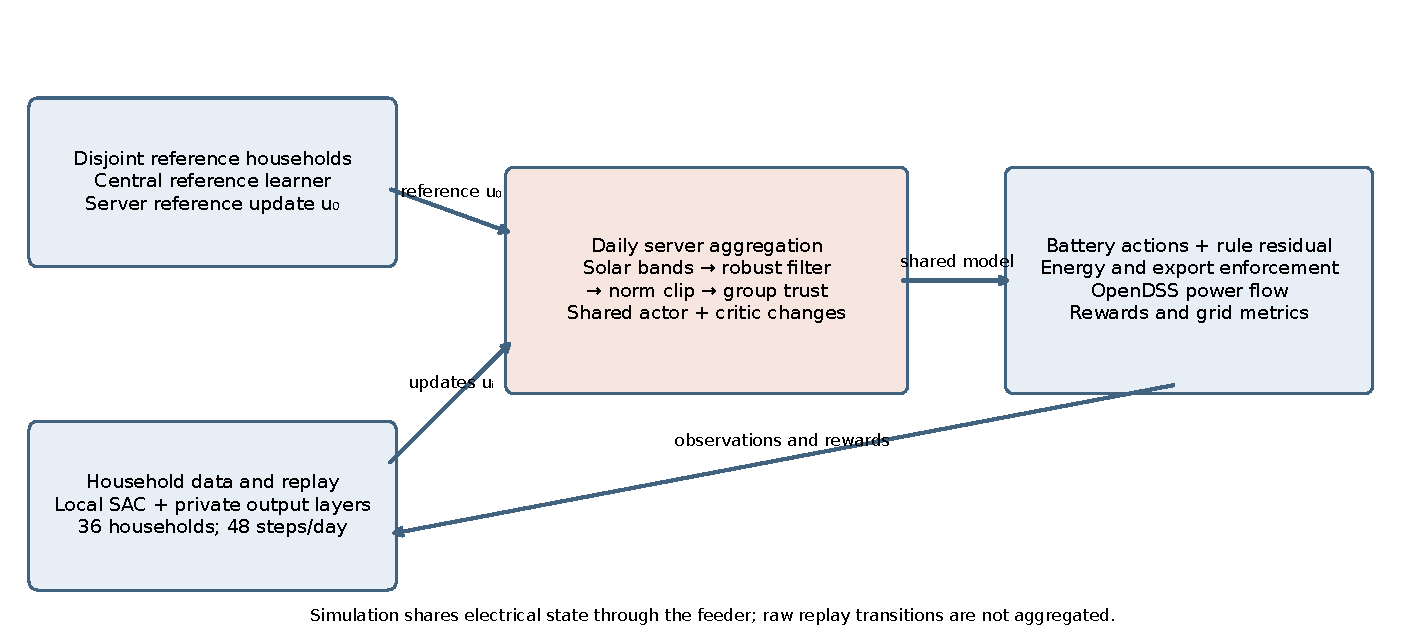
\includegraphics[width=\linewidth]{figures/architecture.pdf}
\caption{Implemented learning and physical-control workflow. Raw replay transitions remain with household learners. The server combines shared parameter changes; a disjoint reference learner provides the trust direction. Export enforcement and power-flow evaluation occur inside the simulator. The reference dataset is an additional trusted resource. Schematic drawn with reproducible Matplotlib code assisted by OpenAI Codex (exact deployed model identifier unavailable).}
\label{fig:architecture}
\end{figure}
\begin{table}[htbp]
\centering\small
\caption{Implemented configuration for the principal case. Tariffs are fixed experimental inputs; MSL denotes minimum system load.}
\label{tab:configuration}
\resizebox{\linewidth}{!}{%
\begin{tabular}{llll}
\toprule
Parameter & Value & Parameter & Value \\
\midrule
Main/scaling households & 36 / 83 & Time step & 0.5 h \\
Solar scale / cap & 6.6 / 10 kWp & Battery capacity & 3 kWh per kWp \\
Battery power & 5 kW & Round-trip efficiency & 0.90 \\
Source voltage & 1.00 pu; stress 1.02 & Voltage bounds & 216.2--253 V \\
Export cap / ordinary floor & 10 / 1.5 kW & MSL export cap & 0 kW \\
Demand trigger & 3660 MW (scenario) & Voltage margin & 1 V \\
Import: 11:00--16:00 & 0.22680 \$/kWh & Import: 16:00--21:00 & 0.45712 \$/kWh \\
Import: other hours & 0.28035 \$/kWh & Export credit & 0.08660 \$/kWh \\
Daily supply charge & 1.48834 \$/day & Curtailment coefficient & 0.08660 \$/kWh \\
Hidden width / batch & 128 / 128 & Learning rate & 0.0003 \\
Discount / target rate & 0.99 / 0.005 & Warmup & 5 days \\
Training / aggregation & 500 days / daily & Shared payload & 54,400 float32 values \\
Solar bands / robust threshold & 3 / 2.5 & Final clipping bound & 2 median norms \\
\bottomrule
\end{tabular}}
\end{table}


\subsection{Battery operation, household exchange and cost}
For household $i$ at time $t$, let $\ell_{i,t}$ denote load, $s_{i,t}$ available photovoltaic power, $p_{i,t}$ battery power (positive for charging), $q_{i,t}$ curtailed solar power and $e_{i,t}$ stored energy. All power quantities use kW. With $\Delta t=0.5$\,h and one-way efficiency $\eta=\sqrt{0.9}$,
\begin{align}
e_{i,t+1}&=e_{i,t}+\Delta t\left[\eta(p_{i,t})^+-(-p_{i,t})^+/\eta\right],\\
g_{i,t}&=\ell_{i,t}+p_{i,t}-s_{i,t}+q_{i,t},
\end{align}
where $(x)^+=\max(x,0)$ and $g_{i,t}>0$ denotes import. Battery capacity is $E_i=3K_i$\,kWh for solar capacity $K_i$\,kWp, and power rating is $P_i=5$\,kW. Requested power is restricted to
\begin{equation}
-\min(P_i,e_{i,t}\eta/\Delta t)\leq p_{i,t}\leq
\min(P_i,(E_i-e_{i,t})/(\eta\Delta t)).
\end{equation}
Half-hour energy cost is
\begin{equation}
c_{i,t}=\Delta t\left[b_t(g_{i,t})^+-f_t(-g_{i,t})^+\right],
\end{equation}
where $b_t$ and $f_t$ denote import and export prices. Annual bills include the fixed daily supply charge. All experiments use the Ergon 12D 2025--26 schedule, including its 16:00--21:00 peak window. The export price is \$0.0866/kWh, consistent with the Queensland Competition Authority's (QCA) corresponding regional feed-in tariff~\cite{qca}; import prices and the supply charge match the retailer's previous rates from 1 July 2025~\cite{ergontariff}. Table~\ref{tab:configuration} lists these fixed inputs.

\subsection{Export schedules and feeder simulation}
OpenDSS solves an unbalanced constant-power snapshot at each half hour. Household reactive demand corresponds to a power factor of 0.98, while photovoltaic generation and batteries operate at unity power factor. The source voltage is 1.00\,pu in the main experiments and 1.02\,pu in the stress case. Voltage penalties use bounds of 216.2--253\,V.

Each daily export schedule is calculated from the actual load and photovoltaic profiles without batteries. Phase-wise voltage sensitivities are estimated by simultaneously increasing export by 1\,kW at each household on a phase. The half-hour schedule uses the most restrictive voltage headroom on that phase and a 1\,V margin below 253\,V. Outside designated minimum-load periods, household allowances are bounded between 1.5 and 10\,kW. This sensitivity-based construction assumes ideal information; it does not solve an optimal power flow or reproduce an operational utility envelope service.

Minimum system load (MSL) periods are selected when the lowest five-minute Queensland demand within a half hour is below 3660\,MW in the archived 2025 series. Mapping the household calendar to that series preserves the weekday and time of day. The 3660\,MW trigger defines the onerous scenario used for the reported MSL charging outcomes; 2600\,MW is a separate typical reference, not the implemented trigger. Export allowances are set to zero in the selected periods.

When requested export exceeds allowance $L_{i,t}$, the simulator first reduces battery discharge and then curtails any remaining excess solar. This enforces $(-g_{i,t})^+\leq L_{i,t}$ under the implemented assumptions. Voltage exceedances can nevertheless remain because of schedule approximation, phase coupling and the ordinary export floor. Peak transformer apparent power is measured relative to nameplate rating, without a hard loading constraint.

\subsection{Residual SAC control}
The self-consumption rule charges from surplus solar and discharges against household demand from 16:00 to 21:00. The learned action is a residual $a_{i,t}\in[-1,1]$:
\begin{equation}
p^{\mathrm{req}}_{i,t}=P_i\operatorname{clip}\left(a^{\mathrm{rule}}_{i,t}+a_{i,t},-1,1\right).
\end{equation}
Battery-energy and export restrictions convert this requested power into executed power. Initialising the deterministic residual at zero recovers the rule, while stochastic warmup actions explore other schedules.

Soft Actor-Critic (SAC) combines reward and entropy maximisation~\cite{sac,sacapps}. Each household observes eleven features: fractional battery charge; scaled current load and photovoltaic power; price; three tariff-period indicators; sine and cosine of time of day; scaled export allowance; and scaled voltage. The actor outputs a Gaussian mean and log standard deviation. Training uses samples transformed by the hyperbolic tangent; evaluation uses the hyperbolic tangent of the Gaussian mean parameter. The actor and twin critics each have two shared hidden layers of width 128 with rectified linear units and a local output layer. Training uses batch size 128, learning rate $3\times10^{-4}$, discount 0.99 and target interpolation coefficient 0.005.

The local reward is
\begin{equation}
r_{i,t}=-c_{i,t}-0.0866\Delta t\,q_{i,t}
-\Delta t\,h_{i,t}-0.1\,v^{\mathrm{out}}_{i,t},
\end{equation}
where $h_{i,t}$ is excess export power after enforcement and $v^{\mathrm{out}}_{i,t}$ is the voltage deviation outside the prescribed interval, in volts. Successful export enforcement makes the export penalty zero. Rewards are multiplied by ten before SAC updates. Because curtailment is penalised in addition to its effect on the bill, the training objective differs from the reported electricity bill.

Training samples seven-day blocks from the training partition. Stored energy carries between days within a block; a newly sampled block starts half charged, and bootstrapping terminates across that discontinuity. Five days of random-action warmup precede learning. The main experiments use 500 training days, with archived 1000-day runs providing additional clean-learning evidence in Table~\ref{tab:extended_clean}. Validation is performed on day 1 and every 25 training days. Central SAC pools household transitions into one agent, whereas local SAC maintains independent agents and replay buffers. These are comparison architectures, not formal performance bounds.

\subsection{Daily federation and FedGrid}
At the end of each training day, households share the actor and critic hidden-layer parameters while retaining their output layers and replay buffers locally. If $\theta_r$ is the server model at round $r$ and $\theta_{i,r}^{\mathrm{local}}$ the shared part after local training, the update is $u_{i,r}=\theta_{i,r}^{\mathrm{local}}-\theta_r$. The server sets $\theta_{r+1}=\theta_r+\mathcal A(\{u_{i,r}\})$ and copies the shared layers to each household. Target critics, optimiser states and entropy temperatures remain local across broadcasts. The shared vector contains 54,400 float32 values, corresponding to 212.5\,KiB per direction per household, excluding protocol overhead.

For FedGrid, solar capacities determine three quantile bands. Medians of update coordinates, norms, distances and absolute deviations use the lower middle order statistic for even-sized samples, matching the implementation; capacity-band boundaries remain quantiles. Any band with fewer than five received updates is merged with a neighbouring band until sufficiently large or only one remains. In group $g$, define a coordinate median $m_g$ and update distances $d_i=\|u_i-m_g\|_2$. Write $\widetilde d_g=\operatorname{median}_{i\in g}d_i$ and
\begin{equation}
\sigma_g=1.4826\operatorname{median}_{i\in g}|d_i-\widetilde d_g|.
\end{equation}
An update passes when $d_i-\widetilde d_g\leq2.5\max(\sigma_g,1.4826\times10^{-12})$. The stabiliser corresponds to flooring the unscaled median absolute deviation before applying the factor 1.4826, as in the implementation. The rule rejects unusually large distances; it does not reject small distances merely because they differ from the median.

In the final configuration, filtering uses the original updates. Admitted updates are then clipped as
\begin{equation}
\widehat u_i=u_i\min\left(1,\frac{2\operatorname{median}_j\|u_j\|_2}{\max(\|u_i\|_2,10^{-12})}\right),
\end{equation}
where the clipping bound uses all received updates, including filtered ones. If $I_g$ is the admitted subset and $\bar u_g=|I_g|^{-1}\sum_{i\in I_g}\widehat u_i$, the group weight and aggregate are
\begin{equation}
w_g=|I_g|\max(0,\cos(\bar u_g,u_0)),\qquad
\mathcal A=\frac{\sum_gw_g\bar u_g}{\max(\sum_gw_g,10^{-12})}.
\end{equation}
Cosine agreement uses the stabilised implementation: each vector norm is floored at $10^{-8}$ before division, so a zero reference or group mean gives zero agreement. The server reference $u_0$ comes from a central learner using a disjoint set of households, starting its shared layers from the current global model each round. A zero total weight produces a zero aggregate. The original FedGrid clips before filtering at one median norm. Therefore, the final revision changes both operation order and clipping multiplier.

\begin{table}[htbp]
\centering
\caption{FedGrid round procedure, matching the final implementation.}
\label{tab:algorithm}
\begin{tabular}{p{0.94\linewidth}}
\toprule
Receive shared changes and household solar bands; train the disjoint reference learner to obtain $u_0$.\\
Merge small bands; compute robust within-band distances on original changes.\\
Mark distance outliers; compute the clipping bound from all received update norms.\\
Clip admitted changes at twice the median norm and form each admitted group mean.\\
Weight group means by admitted size and nonnegative cosine agreement with $u_0$.\\
Apply the weighted aggregate to shared actor and critic layers; retain local output layers.\\
Log outlier-filter decisions separately from any interpretation of effective weight.\\
\bottomrule
\end{tabular}
\end{table}

\subsection{Bounded update size and effective coefficients}
The clipping and nonnegative group weights imply a deterministic bound on the aggregate norm. Let $B=2\operatorname{median}_j\|u_j\|_2$ and $\epsilon=10^{-12}$. Each clipped update has norm at most $B$, and each group mean therefore also has norm at most $B$. With $W=\sum_gw_g\geq0$, the triangle inequality gives
\begin{equation}
\|\mathcal A\|_2\leq\frac{\sum_gw_g\|\bar u_g\|_2}{\max(W,\epsilon)}
\leq B\frac{W}{\max(W,\epsilon)}\leq B.
\end{equation}
This is a deterministic bound on one shared parameter change, not a guarantee on update direction, learning convergence, household cost or physical safety. In particular, an adversary may still change the direction inside the bounded region.

Conditional on a realised set of group weights, the coefficient on an admitted clipped update is
\begin{equation}
\beta_i=\frac{w_{g(i)}}{|I_{g(i)}|\max(W,\epsilon)},
\end{equation}
with $\beta_i=0$ for filtered updates. Filter admission does not imply $\beta_i>0$: a nonpositive group-reference cosine makes $w_{g(i)}=0$. A positive coefficient also does not prove a nonzero causal effect on the eventual action because weights depend on all updates, vectors can cancel, and later policy dynamics intervene. The distinction between admission and positive coefficients motivates reporting them separately. The identities characterise the realised aggregation rule without establishing Byzantine resilience.

\subsection{Comparators and attack model}
The main comparison comprises FedAvg, median, trimmed mean, Krum, FLTrust, FLAME, original and tuned TAFDRL-style filters, and original and final FedGrid. FedProx is additionally evaluated in clean learning. Trimmed mean and Krum receive the assumed compromised share. FLTrust and FedGrid receive the reference learner; comparators therefore do not all use identical auxiliary information. Table~\ref{tab:comparators} summarises their aggregation and admission semantics.
\begin{table}[htbp]
\centering\small
\caption{Comparator scope and admission semantics. Source algorithms are adapted to shared SAC parameter changes; original guarantees are not transferred to this setting.}
\label{tab:comparators}
\resizebox{\linewidth}{!}{%
\begin{tabular}{lll}
\toprule
Method & Aggregation principle & Whole-update rejection statistic \\
\midrule
FedAvg / FedProx & Mean / mean with local proximal term & Not defined \\
Median / trimmed mean & Coordinate statistics & Not defined \\
Krum & Select one neighbour-consistent update & Unselected updates \\
FLTrust & Positive cosine trust; norm rescaling & Zero-trust updates \\
FLAME & Majority clustering, clipping and noise & Outside admitted cluster \\
TAFDRL-style & PCA distance and Beta trust & Distance or minimum-trust exclusion \\
FedGrid & Within-band filter and group trust & Filter exclusion; zero-weight groups omitted \\
\bottomrule
\end{tabular}}
\end{table}


Compromised household positions are sampled for each seed and nominal share and remain fixed within a run. A nominal 30\% share selects 11 of 36 homes. Update attacks preserve local training but replace the transmitted changes. The Normalized attacker observes every honest update, queries the aggregation rule and searches fixed grids for directional mixing and magnitude. Adaptation is therefore limited to that search space. Meter poisoning swaps the learner's load and solar observation channels, while the residual self-consumption rule still uses the simulator's true values; reward poisoning reverses local training rewards. Evaluation uses ordinary observations. Separate message-fault experiments drop or delay honest changes by one round.
\begin{table}[htbp]
\centering\small
\caption{Implemented perturbations. Compromised households are fixed within a run; message faults affect honest households.}
\label{tab:threats}
\resizebox{\linewidth}{!}{%
\begin{tabular}{lll}
\toprule
Threat & Perturbation & Knowledge or scope \\
\midrule
Flip & Negate model changes & Own update \\
Scale & Multiply changes by household count & Own update; system size \\
Noise & Gaussian update variance 1000 & Parameter dimension \\
Normalized & Direction and magnitude grid search & All updates; aggregation queries \\
Meter & Swap observed load and solar channels & Local training observations \\
Reward & Reverse local reward sign & Local training rewards \\
Message faults & 10\% drop and 10\% one-round delay & Honest changes; separate scenario \\
\bottomrule
\end{tabular}}
\end{table}


The model predictive control (MPC) comparator solves a linear program at midnight using exact daily load, solar, prices and export allowances, with a terminal value for stored energy. It is a daily perfect-foresight reference, not a forecast-based controller or an annual global optimum. The program uses separate nonnegative charge and discharge variables and sends their net power to the simulator. A five-day replay check compares the executed bill with the planned bill; the archived implementation does not apply that consistency check throughout the evaluation horizon. Forecast-based MPC and full-horizon validation of this relaxation remain outside the reported experiments.
